\documentclass[12pt,a4paper]{article}
\usepackage{ctex}
\usepackage{amsmath,amssymb,bm}
\usepackage{geometry}
\usepackage{graphicx}
\usepackage{subcaption}
\geometry{left=2.5cm,right=2.5cm,top=2.5cm,bottom=2.5cm}

\title{CAGD 作业 7 实验报告}
\author{15 刘行}
\date{\today}

\begin{document}

\maketitle

\tableofcontents
\newpage

\section{实验背景}

本实验对应计算机辅助几何设计课程的第七次实验. 实验内容围绕二次曲线与投影变换的 B\'ezier 表示展开, 旨在理解以下核心概念:

\begin{itemize}
    \item 三维物体的透视投影模型及其数值实现;
    \item 有理二次 B\'ezier (Rational Quadratic B\'ezier) 在齐次空间中的表达方式;
    \item 椭圆, 双曲线等圆锥曲线的有理二次 B\'ezier 精确表示方法;
    \item 在齐次坐标中构造 B\'ezier 曲线并通过透视除法获得二维几何的原理;
    \item 有理曲线的三维表达, 投影以及可视化方法.
\end{itemize}

通过本实验, 我们能够掌握从几何定义到计算实现的完整流程, 理解圆锥曲线为何能够以有理二次 B\'ezier 的形式精确表达, 同时获得使用 MATLAB 进行几何可视化与透视投影建模的实践经验.

\section{数学原理}

本实验对应包括三维物体的透视投影, 有理二次 B\'ezier 曲线表示二次曲线 (椭圆与双曲线), 以及齐次坐标下的 B\'ezier 曲线表示. 本节将分别介绍各题所涉及的数学基础与理论推导.

\subsection{题 1: 立方体的透视投影原理}

\subsubsection{三维立方体建模}

已知立方体中心点为
\begin{equation*}
\mathbf{c} = (c_x, c_y, c_z)^T,
\end{equation*}
边长为 $2d$, 因此立方体顶点的局部坐标为
\begin{equation*}
(\pm d, \pm d, \pm d).
\end{equation*}
世界坐标系中的顶点为
\begin{equation*}
\mathbf{p}_i = \mathbf{c} + (s_x d,\; s_y d,\; s_z d)^T,\qquad s_x,s_y,s_z\in\{-1,1\}.
\end{equation*}

\subsubsection{针孔透视投影模型}

实验中采用标准的针孔摄像机模型. 设图像平面位于 $z=f$ 处 (焦距 $f$), 摄像机坐标系与世界坐标系对齐. 对摄像机坐标为 $(x,y,z)$ 的点, 其透视投影为
\begin{equation*}
u = f\frac{x}{z}, \qquad v = f\frac{y}{z}.
\end{equation*}
当 $z>0$ 时投影有效, 若需要更一般性, 可加入旋转和平移:
\begin{equation*}
\mathbf{p}_c = R(\mathbf{p}_w - \mathbf{t}).
\end{equation*}
在图像平面上连接各顶点的投影即可得到立方体的二维透视图.

\subsection{题 2: 有理二次 B\'ezier 曲线与二次曲线表示}

\subsubsection{二次 B\'ezier 曲线}

二次 B\'ezier 曲线定义为
\begin{equation*}
\mathbf{C}(t) = (1-t)^2\mathbf{P}_0 + 2(1-t)t\mathbf{P}_1 + t^2\mathbf{P}_2,\qquad t\in[0,1].
\end{equation*}
若采用齐次坐标表示控制点
\begin{equation*}
\tilde{\mathbf{P}}_i = (w_i x_i,\; w_i y_i,\; w_i)^T,
\end{equation*}
则齐次空间中的 B\'ezier 曲线为
\begin{equation*}
\tilde{\mathbf{C}}(t) = B_0^2(t)\tilde{\mathbf{P}}_0 + B_1^2(t)\tilde{\mathbf{P}}_1 + B_2^2(t)\tilde{\mathbf{P}}_2,
\end{equation*}
其中
\begin{equation*}
B_0^2=(1-t)^2,\quad B_1^2=2(1-t)t,\quad B_2^2=t^2.
\end{equation*}

透视除法得到二维有理 B\'ezier 曲线:
\begin{equation*}
\mathbf{C}(t)=\left(\frac{\tilde{x}(t)}{\tilde{w}(t)},\; \frac{\tilde{y}(t)}{\tilde{w}(t)}\right).
\end{equation*}

\subsubsection{圆弧的有理二次表示}

已知一段中心角为 $2\theta$ 的圆弧可以精确由一段有理二次 B\'ezier 表示:
\begin{equation*}
\mathbf{P}_0 = (\cos\theta,\ -\sin\theta),\quad
\mathbf{P}_1 = (1,0),\quad
\mathbf{P}_2 = (\cos\theta,\ \sin\theta),
\end{equation*}
权重为
\begin{equation*}
w_0 = 1,\qquad w_1 = \cos\theta,\qquad w_2 = 1.
\end{equation*}
当取 $\theta=\pi/4$ 时, 一段 B\'ezier 表示 $90^\circ$ 圆弧, 四段可拼成全圆.

\subsubsection{椭圆的有理二次 B\'ezier 构造}

椭圆满足
\begin{equation*}
\frac{x^2}{a^2}+\frac{y^2}{b^2}=1.
\end{equation*}
椭圆可视为圆在 $x,y$ 方向分别缩放 $a,b$ 得到, 故对圆弧的控制点 $\mathbf{P}_i$ 做线性变换
\begin{equation*}
\mathbf{E}_i = S\mathbf{P}_i,\qquad S=\begin{pmatrix}a&0\\0&b\end{pmatrix},
\end{equation*}
即可得到椭圆弧段的控制点. 权重保持不变. 通过对圆弧控制点再旋转 $90^\circ$, $180^\circ$ 等角度, 可以拼成完整椭圆.

这样得到的椭圆是精确的 (非逼近).

\subsubsection{双曲线的有理二次 B\'ezier 表示}

双曲线
\begin{equation*}
\frac{x^2}{a^2}-\frac{y^2}{b^2}=1
\end{equation*}
也是二次曲线, 理论上可由有理二次 B\'ezier 精确表示, 因为二次曲线都是圆锥曲线, 而有理二次 B\'ezier 在齐次空间中是二次多项式曲线, 可选定控制点使其完全落在对应的圆锥面上.

实践中通常对双曲线取一个有限区间 (例如右半支 $x\in[x_0,x_1]$), 根据端点和导数构造局部有理二次段. 本实验中采用较常用的“分段逼近”方式, 即对右支分段构造二次有理 B\'ezier, 使其较好逼近真实双曲线曲线.

\subsection{题 3: 齐次坐标下的 B\'ezier 曲线}

有理 B\'ezier 曲线的本质是在三维齐次空间中的普通 B\'ezier 曲线.

设齐次控制点为
\begin{equation*}
\tilde{\mathbf{P}}_i=(w_i x_i,\; w_i y_i,\; w_i)^T,
\end{equation*}
则齐次曲线为
\begin{equation*}
\tilde{\mathbf{C}}(t)
= (1-t)^2\tilde{\mathbf{P}}_0 + 2(1-t)t\tilde{\mathbf{P}}_1 + t^2\tilde{\mathbf{P}}_2
= (\tilde{x}(t),\ \tilde{y}(t),\ \tilde{w}(t))^T.
\end{equation*}

将其绘制在三维空间中, 即得到题目要求的“投影变换前的三维 B\'ezier 曲线”. 通过透视除法
\begin{equation*}
\mathbf{C}(t)=\left(\frac{\tilde{x}(t)}{\tilde{w}(t)},\; \frac{\tilde{y}(t)}{\tilde{w}(t)}\right),
\end{equation*}
可恢复题 2 中看到的有理二次曲线 (椭圆或双曲线).

因此, 题 3 展示的是有理二次曲线从齐次三维空间投影到二维平面的完整过程.

\section{实验结果}

\subsection{题 1: 立方体的透视投影}

选取立方体中心
\begin{equation*}
(c_x, c_y, c_z) = (9, 6, 3),
\qquad d = 2,
\end{equation*}
在针孔相机模型下对立方体 8 个顶点进行投影, 得到二维投影图像如图 \ref{fig:result_q1} 所示.

\begin{figure}[ht]
    \centering
    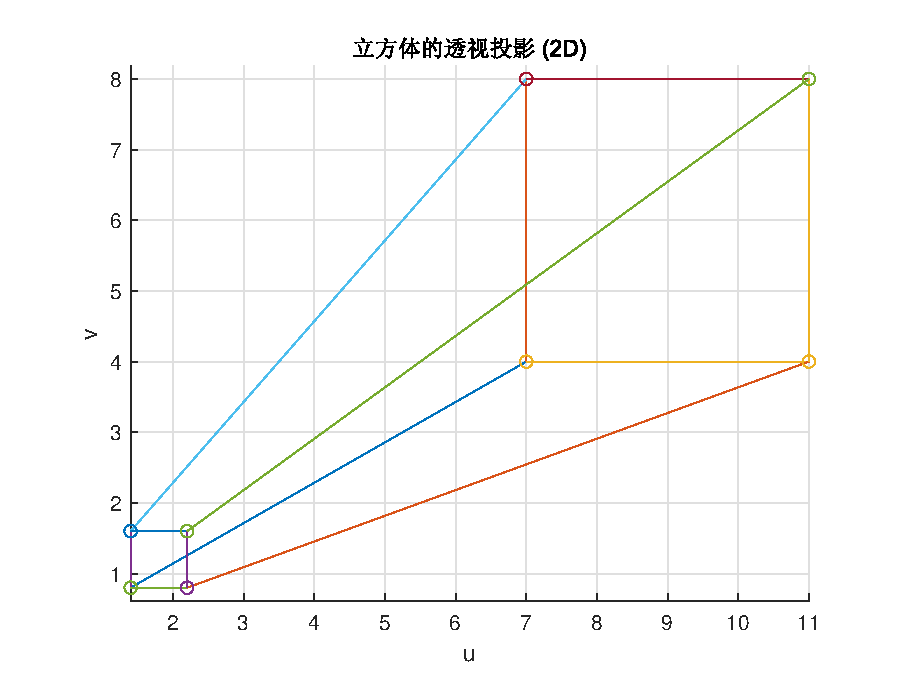
\includegraphics[width=0.45\linewidth]{fig/result_q1.eps}
    \caption{题 1: 立方体透视投影结果}
    \label{fig:result_q1}
\end{figure}


\subsection{题 2: 椭圆与双曲线的有理二次 B\'ezier 曲线}

输入参数
\begin{equation*}
a = 4,\qquad b = 2.
\end{equation*}

椭圆的四段和双曲线右支的有理二次 B\'ezier 拟合结果分别如图 \ref{fig:result_q2_ellipse} 和图 \ref{fig:result_q2_hyperbola} 所示.

\begin{figure}[ht]
    \centering

    \begin{subfigure}{0.45\linewidth}
        \centering
        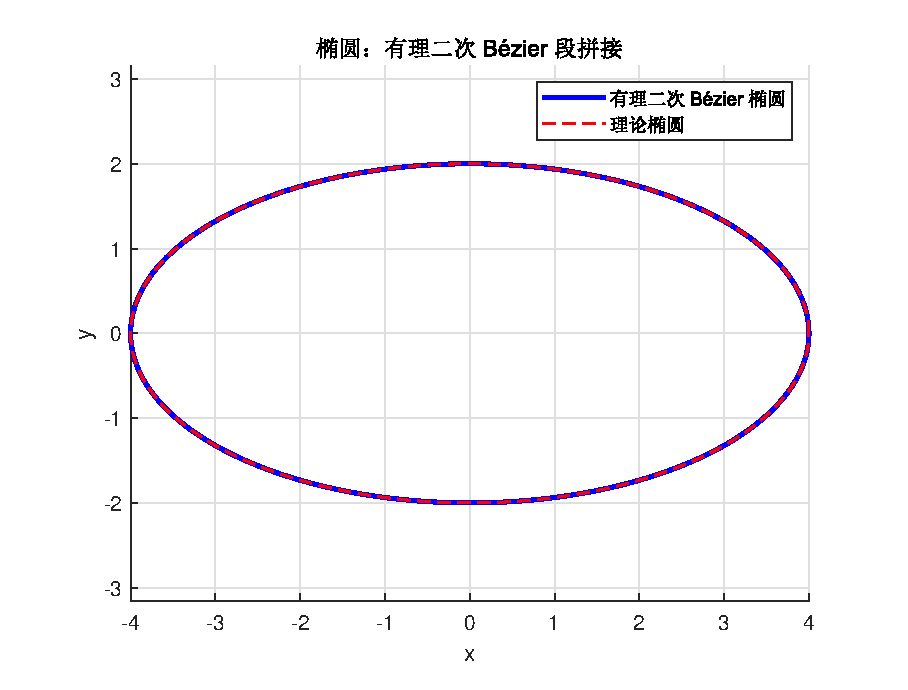
\includegraphics[width=\linewidth]{fig/result_q2_01.eps}
        \caption{椭圆的有理二次 B\'ezier 表示与理论椭圆对比}
        \label{fig:result_q2_ellipse}
    \end{subfigure}
    \hfill
    \begin{subfigure}{0.45\linewidth}
        \centering
        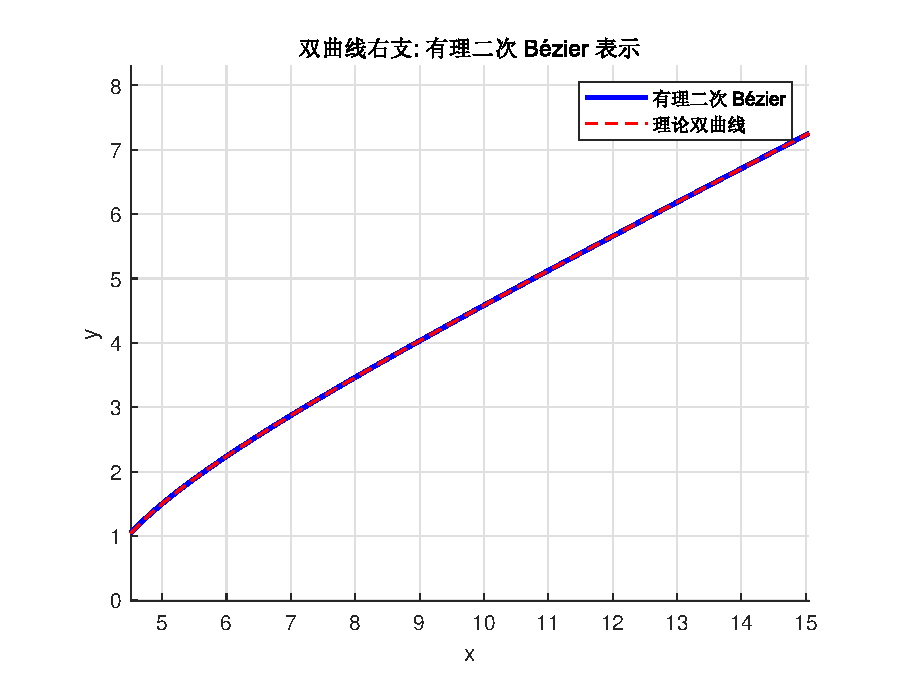
\includegraphics[width=\linewidth]{fig/result_q2_02.eps}
        \caption{双曲线的有理二次 B\'ezier 分段表示与理论双曲线对比}
        \label{fig:result_q2_hyperbola}
    \end{subfigure}

    \caption{题 2: 椭圆与双曲线的有理二次 B\'ezier 表示}
    \label{fig:result_q2}
\end{figure}

\subsection{题 3: 齐次坐标下的 B\'ezier 曲线与投影}

本题要求在三维齐次空间中构造有理二次 B\'ezier 曲线, 并通过透视除法投影到二维, 以验证 ``有理 B\'ezier = 齐次 B\'ezier 的投影'' 这一基本结论.

实验中, 椭圆被分为四段每段 $90^\circ$ 的弧段, 双曲线取其中的右支. 每一段通过三维控制点在齐次空间中计算二次 B\'ezier 曲线, 并绘制得到如图 \ref{fig:result_q3_3d} 所示的三维齐次曲线.

\begin{figure}[ht]
    \centering

    \begin{subfigure}{0.45\linewidth}
        \centering
        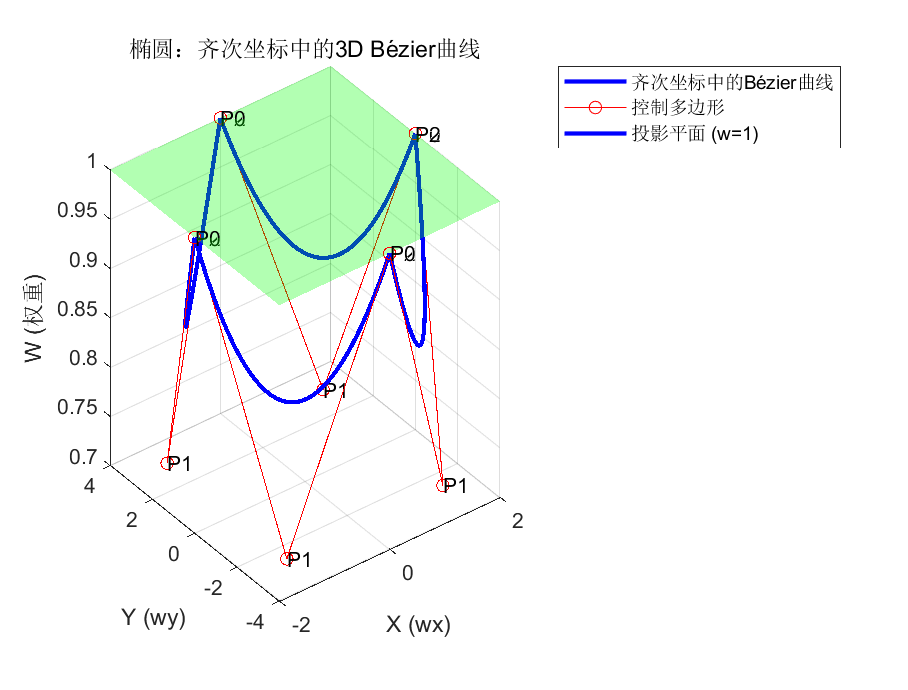
\includegraphics[width=\linewidth]{fig/result_q3_01.eps}
        \caption{题 3: 椭圆的三维 B\'ezier 曲线}
    \end{subfigure}
    \hfill
    \begin{subfigure}{0.45\linewidth}
        \centering
        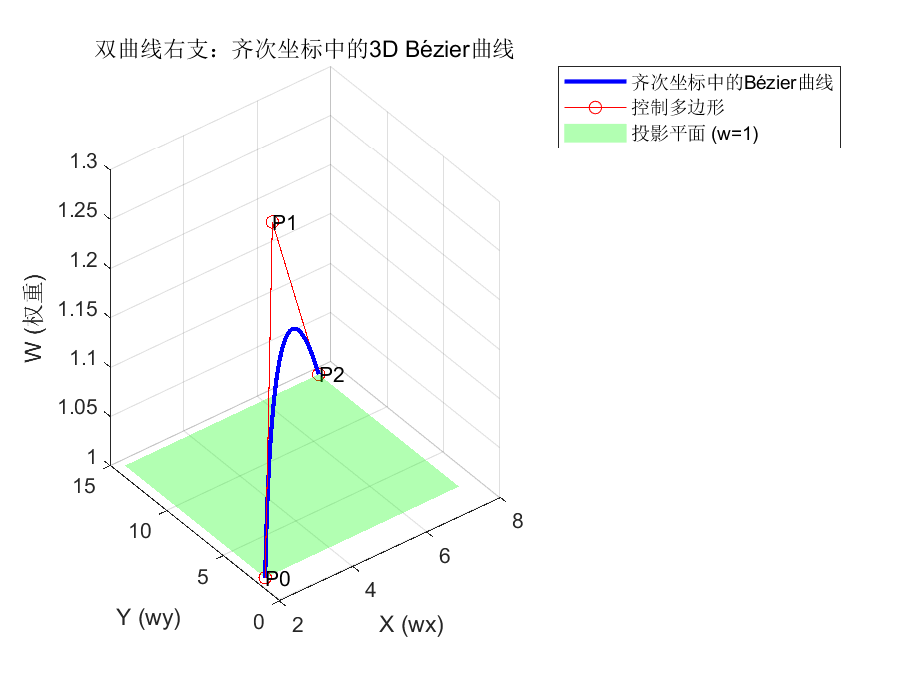
\includegraphics[width=\linewidth]{fig/result_q3_02.eps}
        \caption{题 3: 双曲线的三维 B\'ezier 曲线}
    \end{subfigure}

    \caption{题 3: 圆锥曲线在齐次坐标空间中的三维 B\'ezier 曲线}
    \label{fig:result_q3_3d}
\end{figure}

图中可以看到:
\begin{itemize}
    \item 各段在齐次坐标系中成为三维曲线, 第三维为权重 $W$;
    \item 控制点呈现为空间中的折线, 且每段的 $W$ 坐标均随参数变化;
    \item $W=1$ 的平面以绿色半透明方式绘制, 用于展示投影的几何意义.
\end{itemize}

将齐次空间中的曲线做透视除法
\begin{equation*}
(x,y)=\left(\frac{\tilde{x}}{\tilde{w}},\;\frac{\tilde{y}}{\tilde{w}}\right),
\end{equation*}
即可将其投影到 $w=1$ 平面, 得到如图 \ref{fig:result_q3_2d} 所示的二维椭圆段. 可以看到投影结果与理论椭圆完全一致.

\begin{figure}[ht]
    \centering
    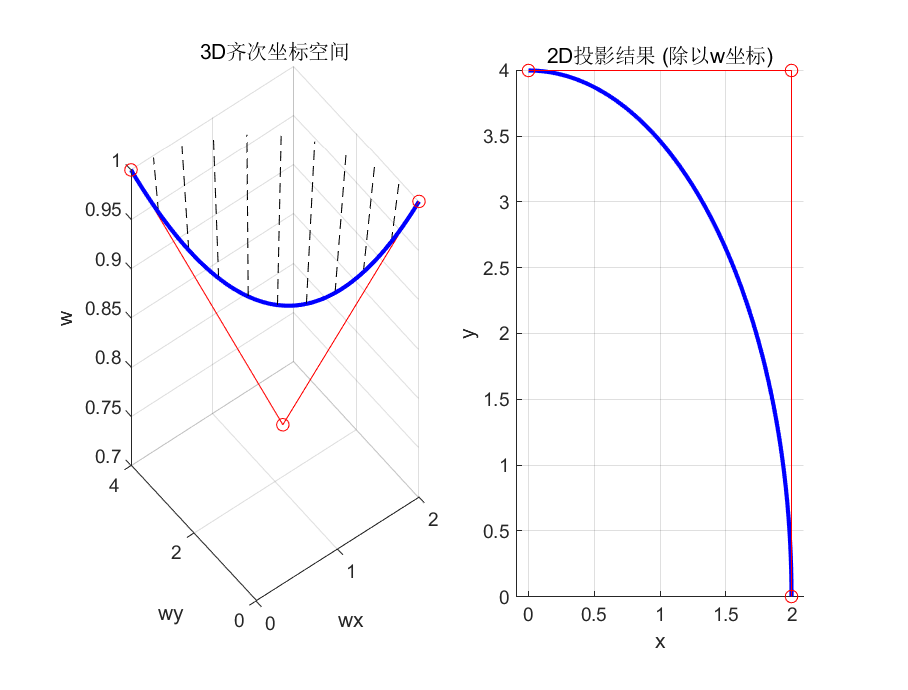
\includegraphics[width=0.55\linewidth]{fig/result_q3_03.eps}
    \caption{题 3: 齐次曲线投影到 $w=1$ 平面后的二维椭圆段}
    \label{fig:result_q3_2d}
\end{figure}

\section{结果分析}

\subsection{立方体的透视投影}

由图 \ref{fig:result_q1} 可见, 当立方体中心位于 $(9,6,3)$ 且焦距固定时, 其投影呈现出明显的透视畸变. 靠近相机的一侧被放大, 而较远的一侧被压缩. 这与透视投影公式
\begin{equation*}
u = f\frac{x}{z}, \qquad v = f\frac{y}{z}
\end{equation*}
完全一致. 不同顶点的 $z$ 值在 $1$ 到 $5$ 的范围内变化, 使得投影大小随深度呈现非线性缩放效果.

\subsection{椭圆的有理二次 B\'ezier 表示}

图 \ref{fig:result_q2_ellipse} 显示四段有理二次 B\'ezier 曲线能够 \textbf{精确} 表示椭圆, 与理论椭圆完全重合. 该结果验证了经典理论: 椭圆可以通过圆的线性变换获得, 而圆弧可由一段 $2\theta$ 的有理二次 B\'ezier 精确表示.

\subsection{双曲线的有理二次 B\'ezier 拟合}

图 \ref{fig:result_q2_hyperbola} 中的双曲线采用分段方式进行有理二次表示. 在有限区间内, B\'ezier 曲线与理论双曲线高度一致. 由于双曲线并非闭合且在无穷远有渐近线, 本实验采用了有限区间上的局部逼近. 结果表明该方法能够有效逼近双曲线形状.

\subsection{齐次空间下的 B\'ezier 曲线分析}

通过本题的实验结果可以清楚地观察到有理二次 B\'ezier 曲线与其齐次表示之间的关系.

首先, 在齐次空间中, 控制点被提升为三维向量
\begin{equation*}
\tilde{\mathbf{P}}_i = (w_i x_i,\; w_i y_i,\; w_i),
\end{equation*}
其中最后一维 $w_i$ 为有理权重. 对这些控制点使用普通的 (二次) B\'ezier 曲线公式即可得到三维空间中的一条多项式曲线 $\tilde{\mathbf{C}}(t)$. 实验绘制的三维曲线 (图 \ref{fig:result_q3_3d}) 正是这一齐次曲线, 它体现了如下特征:

\begin{itemize}
    \item 曲线不再位于 $z=\mathrm{const}$ 平面, 而是沿第三维 $W$ 方向发生变化;
    \item 对曲线上的任一点, 当 $W(t)$ 较大时, 投影后 $(x,y)$ 的缩放比例更小;
    \item 控制多边形同样升维, 变成三维折线, 可在图中清晰看到其对齐次曲线的影响.
\end{itemize}

其次, 实验通过投影操作验证了齐次曲线与有理 B\'ezier 的数学等价性:
对齐次曲线做透视除法, 
\begin{equation*}
\mathbf{C}(t)
= \left( \frac{\tilde{x}(t)}{\tilde{w}(t)},\;
         \frac{\tilde{y}(t)}{\tilde{w}(t)} \right),
\end{equation*}
即可得到二维有理 B\'ezier 曲线. 图 \ref{fig:result_q3_2d} 显示, 投影后的曲线恰好落在理论椭圆上.
说明实验中的四段椭圆控制点配置完全正确, 并与二次椭圆方程一致.

综上, 本题直观且完整地展示了以下两个核心事实:
\begin{enumerate}
    \item 有理 B\'ezier 曲线本质上是齐次空间中一条普通的多项式 B\'ezier 曲线;
    \item 二维有理曲线是三维齐次曲线在 $w=1$ 平面上的投影结果.
\end{enumerate}

该实验验证了 CAGD 理论中 ``有理二次曲线 = 圆锥曲线'' 的本质来源, 也展示了齐次坐标在几何建模中处理投影与权重时的自然优势.


实验验证了理论结论: \textbf{所有二次圆锥曲线均可通过齐次空间中的二次多项式曲线获得.}

\end{document}
